\documentclass[Main]{subfiles}
\begin{document}

\chapter{Prototype: DDS}


\section{Design and architecture}
Setting up 2 publishers and 2 subscribers will give an idea of how a DDS system can be used.
In this example the two cities Gotham and Metropolis acting as publishers, have citizens reporting different kind of emergencies.
Citizen can, as topic, report a bar fight, a blood clot, a break in and a paper cut.
The Police Station and the Medic Station acts as subscribers to the events but will not respond to any call.


\begin{figure}[hbtp]
\centering
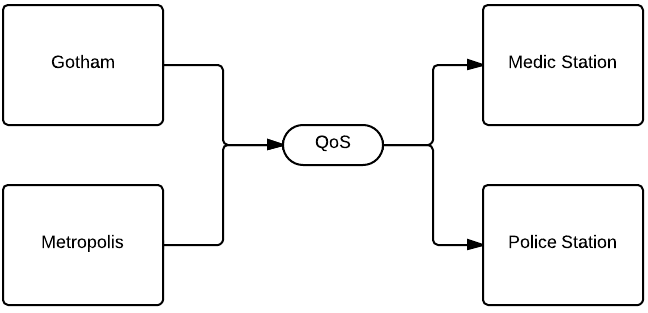
\includegraphics[scale=0.6]{DDSChart}
\caption{Design of prototype.}
\label{Fig:pub-sub}
\end{figure}

The QoS registers all emergencies and the sends the messages to the stations as shown in Table \ref{tab:emergencies}.

\begin{table}[htbp]
\centering

\begin{tabular}{l|c|c}
 & Medic Station & Police Station \\ 
\hline 
Paper cut & - & - \\ 
Break in & - & + \\ 
Bar fight & + & + \\ 
Blood clot & + & - \\ 
\hline 
\end{tabular} 

\caption{Stations will move out to '+' but not '-'.}
\label{tab:emergencies}
\end{table}

As shown in Table \ref{tab:emergencies} the Medic Station will move out to bar fights and blood clots but no paper cuts and break ins.
The Police Station will however move out to break ins and bar fights but not blood clots and paper cuts.

The program first start the two subscribers and afterwards the two publishers.
Typing in a category, a message and a key in the publisher will send it to the QoS and let it show in the subscribers if they subscribe to the category as shown in Figure \ref{Fig:example}.


\begin{figure}[hbtp]
\centering
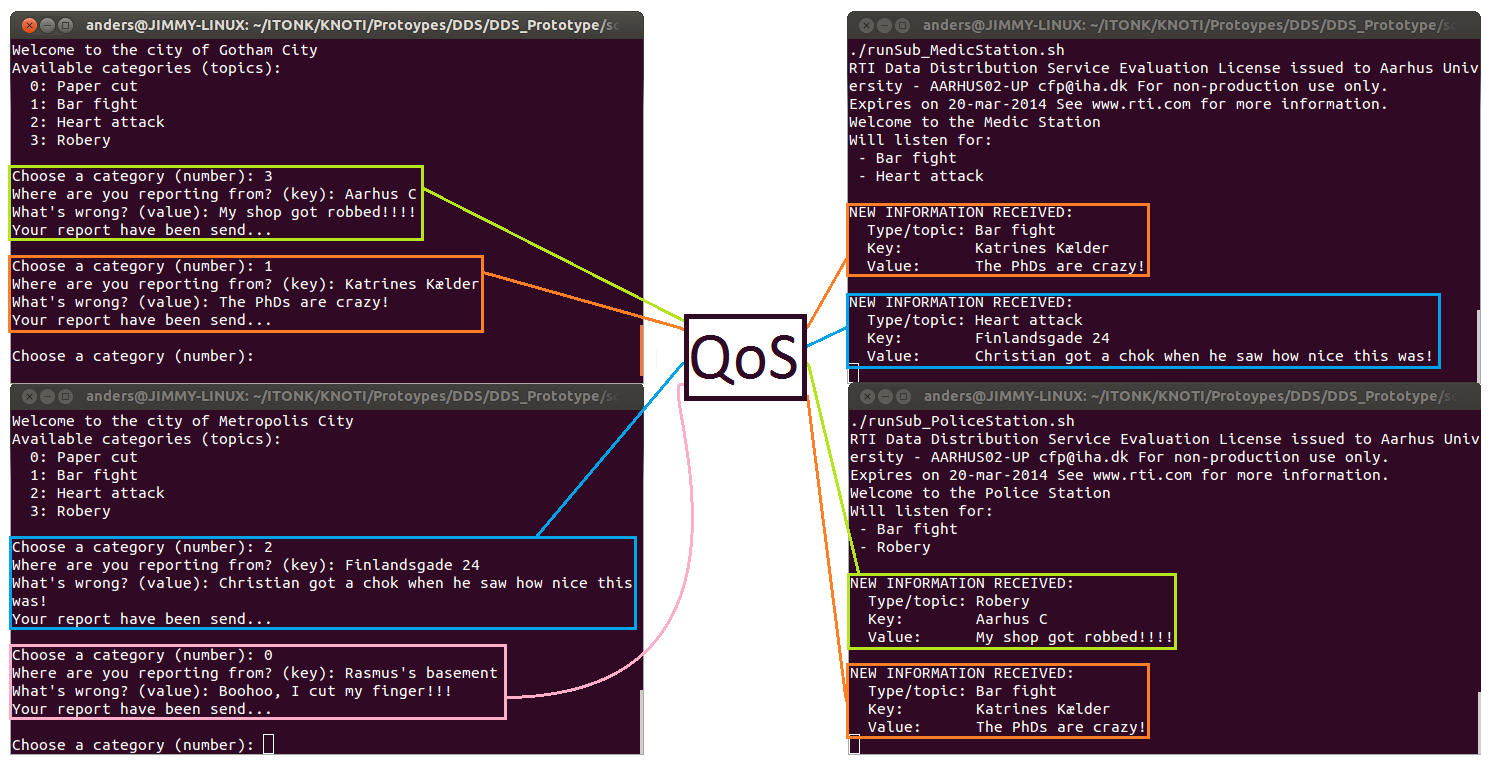
\includegraphics[scale=0.3]{ConsoleExample}
\caption{Console windows of 2 subscribers and 2 publishers}
\label{Fig:example}
\end{figure}


Attached to the document is the project files, where all the \code{.sh}-files are compiled.
Running the 2 subscribers will let them start listing for topics.
Running the 2 publishers let the user decided which topics they will publish.
After the topics have been selected the publishers can sends message's key and the message's actual message.

When the message is sent it will written in the console of the subscriber(s).




\section{The implementation}

The implementation is split up in to four files, each providing its own service for the program to start.

	\begin{itemize}
	\item \textbf{RTIHelper.java}
	\\
	Provides different helper methods for both the publisher and the subscriber

	\item \textbf{ReportListener.java}
	\\
	Provides the listener functionality to the middleware to send the data for the subscriber.
	
	\item \textbf{ReportSubscriber.java}
	\\
	Takes a name for a station and optional numbers of topics to subscribe to as argument. Will call the \code{ReportListener.java} to attach it self.
	
	\item \textbf{CityPublisher.java}
	\\
	Takes one argument as a name of the city. 
	Creates a topic and a datawriter from \code{ReportListener.java} and reads user input for messages.
	
	\end{itemize}

The \code{RTIHelper} contains four methods:

\begin{lstlisting}[caption=RTIHelper: getDomain(), style=Code-Java, label=lst:getDomain]
static DomainParticipant getDomain() {
	return DomainParticipantFactory.get_instance().create_participant(
			0, // Domain ID = 0
			DomainParticipantFactory.PARTICIPANT_QOS_DEFAULT, 
			null, // no listener
			StatusKind.STATUS_MASK_NONE);
}
\end{lstlisting}

\codeTitle \ref{lst:getDomain} creates a new domain participant which is the reference to the domain, here with the \code{ID} predefined to '0'.
Furthermore it specifies which QoS must be attached to the participant though the \code{PARTICIPANT\_QOS\_DEFAULT} is chosen here for simplicity.
The domain has no listeners and therefore the mask is \code{STATUS\_MASK\_NONE}.

\begin{lstlisting}[caption=RTIHelper: createTopic, style=Code-Java, label=lst:createTopic]
static Topic createTopic(DomainParticipant domain, String topicStr) {
	return domain.create_topic(
			topicStr, 
			KeyedStringTypeSupport.get_type_name(), 
			DomainParticipant.TOPIC_QOS_DEFAULT, 
			null, // no listener
			StatusKind.STATUS_MASK_NONE);
}
\end{lstlisting}


\codeTitle \ref{lst:createTopic} creates a new topic that can be used for both publishers and subscribers. 
The only thing that differs the different topics in the prototype are their names, defined for the first parameter.
 This is the one equal to e.g. "Robery" or "Bar fight". 
 Via the last parameters it is told that the topic is bound to the \code{KeyedString} type, the default QoS because of simplicity is used for creating the topic and that there like for the \code{DomainParticipant} won't be any listeners. 

\begin{lstlisting}[caption=RTIHelper: createKeyedStringWriter, style=Code-Java, label=lst:createKeyedStringWriter]
static KeyedStringDataWriter createKeyedStringWriter(DomainParticipant domain, Topic topic) {
	DataWriter writer = domain.create_datawriter(
				topic, 
				Publisher.DATAWRITER_QOS_DEFAULT,
				null, // no listener
				StatusKind.STATUS_MASK_NONE);
	return (KeyedStringDataWriter) writer;
}
\end{lstlisting}

\code{DataWriter} is created based on a previously created topic. 
Default QoS  is used and there isn't any listeners.


\begin{lstlisting}[caption=RTIHelper: createKeyedStringReader, style=Code-Java, label=lst:createKeyedStringReader]
static KeyedStringDataReader createKeyedStringReader(DomainParticipant domain, ReportListener listener, Topic topic) {
	DataReader reader = domain.create_datareader(
				topic, 
				Subscriber.DATAREADER_QOS_DEFAULT,
				listener,         // Listener
				StatusKind.DATA_AVAILABLE_STATUS);
	return (KeyedStringDataReader) reader;
} 
\end{lstlisting}

\code{DataReader} is created based on a previously made topic and are using default QoS. 
It is specified that a listener is bound to the reader, so it will be called every time new data is available. 
The listener in this prototype is the \code{ReportListener}.



\end{document} 